\documentclass{report}
\usepackage[T1]{fontenc}
\usepackage[utf8]{inputenc}
\usepackage[french]{babel}
\usepackage{color}
\usepackage{amsmath}
\usepackage{amssymb}
% Pour utiliser le signe €
\usepackage{eurosym}
% Pour pouvoir insérer des images
\usepackage{graphicx}
\graphicspath{images/}
% Pour pouvoir insérer des hyperliens
\usepackage[hyphens]{url}
\usepackage{hyperref}
% Suppression des marges supplémentaires sur les bords
\usepackage{fullpage}
% Forcer l'affichage des figures à un endroit précis
\usepackage{here}
% On ne veut pas afficher le mot 'Chapitre' avant chaque chapitre
\usepackage{titlesec}
\titleformat{\chapter}[hang]{\bf\huge}{\thechapter}{2pc}{}

% Pour les en-têtes et pieds de page
\usepackage{fancyhdr}
\renewcommand{\headrulewidth}{0pt}
\lhead{} 
\chead{} 
\rhead{} 
\renewcommand{\footrulewidth}{0pt}
\lfoot{Antoine Augusti} 
\cfoot{\thepage} 
\rfoot{statistics.teen-quotes.com} 
\pagestyle{fancy}

% Coloration syntaxique
\usepackage{listings}
\lstset{ 
	language=PHP,
	numbers=left,
	showstringspaces=false, 
	tabsize=4,
	breaklines=true,
	extendedchars=true,
	literate={é}{{\'e}}1 {à}{{\'a}}1 {è}{{\`e}}1 {ç}{{\c c}}1
}
%----------------------- %
% -- Cheat sheet -------- %

% Alignement
%\begin {flushleft}
%\begin {center}
%\begin {flushright}

% Listes
% \begin{itemize}
% \begin{description}
% \begin{enumerate}
% 	\item Numéro 1
% 	\item Numéro 2
% \end{enumerate}
% \\
% \newpage

% Mise en forme des caractères
% \normalfont{} ou \begin{rm}
% \textbf{} ou \begin{bf}
% \textit{} ou \begin{it}
% \textsc{} ou \begin{sc}
% Emphase (sémantique)
% \emph{}

% Citations et code brut
% \quote Pour une ligne isolée
% \quotation Pour un bloc
% \verb Pour du code
% \lstlisting Pour du code coloré

% URL
% \url{http://www.site.org/}
% ------------------------------------ %


% ------------------------------------ %
% -- METADONNÉES DU DOCUMENT --------- %
% Utilisées pour générer la page de garde
\title{
		Projet Final de M8\\
		Étude de Teen Quotes
}
\author{
	Antoine \textsc{Augusti}, 
}
\date{Juin 2013}

\begin{document}

	% Génération de la page de garde
	\maketitle

	% Génération de la table des matières
	\tableofcontents

	% ///////////////////////////////////////////////////////// %
	% /// Introduction //////////////////////////////////////// %
	\chapter{Introduction}
	% ------------------------------------------- %
	% -- Teen Quotes, qu'est-ce que c'est ? ----- %
	\section{Teen Quotes, qu'est-ce que c'est ?}
	Teen Quotes est une plateforme regroupant des citations décrivant le quotidien des adolescents. L'adolescence est une période difficile à gérer dans la vie et les adolescents ont souvent besoin d'échanger autour de sujets qui les préoccupent : leurs amis, l'amour, les études, leurs déceptions, leurs expériences. Teen Quotes répond à ce besoin en proposant à toute personne possédant un compte de pouvoir partager son impression en écrivant une courte citation. Cette citation sera ensuite acceptée (modifiée légèrement ou non) pour publication ou rejetée. Actuellement, cinq nouvelles citations sont publiées tous les jours à 0h (heure française) sur Teen Quotes.\\

	L'interface de Teen Quotes est proposée par défaut en anglais. L'interface est également disponible en français pour ceux qui le désirent et une version en français par défaut existe (elle se nomme Kotado). Toutefois, la version française de Teen Quotes ayant moins de succès que la version originale, j'ai choisi d'orienter mon projet de M8 vers cette version anglaise.\\

	Teen Quotes a été lancé en mai 2011, après quelques mois de développement que j'ai mené seul. Aujourd'hui Teen Quotes possède une version web pour les ordinateurs, une version optimisée pour les smartphones (depuis navigateur) ainsi qu'une application iPhone / iTouch que l'on peut télécharger depuis l'App Store d'Apple. \textbf{Plus de 1,5 million de personnes ont visité Teen Quotes}, depuis l'une des versions que nous proposons.\\

	Je me suis également associé depuis deux ans à une jeune femme philippine (parlant anglais) qui tient le compte Twitter de Teen Quotes (\href{http://twitter.com/ohteenquotes}{\textit{@ohteenquotes}}) comptant actuellement \textbf{plus de 2 millions de followers}. Nous essayons ensemble d'avoir une convergence vers tous les supports où Teen Quotes est présent (Twitter, Facebook, site web, site mobile, application iPhone / iTouch) pour agrandir notre masse d'utilisateurs.

	% ---------------------------------------------------- %
	% -- Et moi, je peux avoir accès à Teen Quotes ? ----- %
	\section{Et moi, je peux avoir accès à Teen Quotes ?}
	Bien évidemment ! Teen Quotes est ouvert à tout le monde et mon but est que le plus de monde possible rejoigne l'aventure. Teen Quotes peut être consulté grâce aux moyens suivants :
	\vspace{10px}
	\begin{itemize}
		\item Site web : \url{http://teen-quotes.com}
		\item Site mobile \footnote{Lien à visiter depuis un smartphone ou une tablette. La redirection vers la version mobile est automatique quand on tente de visiter le site classique depuis un smartphone ou une tablette.} : \url{http://m.teen-quotes.com}
		\item Application iPhone / iTouch \footnote{Lien à visiter depuis un iPhone ou un iTouch pour lancer le téléchargement de l'application !} : \url{http://teen-quotes.com/apps}
	\end{itemize}

	% ---------------------------------------------------- %
	% -- Des données oui, mais des données à jour -------- %
	\section{Des données oui, mais des données à jour}
	Teen Quotes enregistre plus de \textbf{4 000 visites par jour}. Les bases de données de Teen Quotes enregistrent environ \textbf{30 000 requêtes par heure}. Avec un tel volume de données, difficile de se contenter d'une étude statistique figée, obslète une semaine plus tard car les données ne sont plus du tout les mêmes. Teen Quotes est vivant, évolue en permanence : l'étude statistique de Teen Quotes doit s'adapter en conséquence.\\

	En réponse à ce défi, j'ai décidé d'orienter mon projet de M8 vers une étude statistique évolutive, qui se renouvelle en permanence et qui a pour ambition de donner des informations correctes et précises en quasi temps réel. Pour répondre à ce besoin, quoi de mieux que de proposer une étude en ligne ? Facile à consulter : il suffit d'un navigateur web.

	% Comment ça fonctionne ?
	\subsection{Comment ça fonctionne ?}
	L'idée était donc de créer une partie du site de Teen Quotes dédiée aux statistiques : affichage de graphiques et informations sur les données. Les données sont recalculées 3 fois par heure (soit \textbf{toutes les 20 minutes} si vous suivez !). La réflexion suivie pour arriver à ceci a donc été la suivante :
	\vspace{10px}
	\begin{enumerate}
		\item Quelles sont les données que je veux afficher ?
		\item Comment est-ce que je peux récupérer ces données ? Sont-elles enregistrées dans mes bases de données ou sur un service externe (Google Analytics \footnote{Google Analytics fournit une analyse d'audience pour le site web classique et le site web mobile.}, Flurry \footnote{Flurry fournit des données sur les utilisateurs de l'application iPhone / iTouch.}) ?
		\item Comment faut-il rassembler les données ? Comment donner du sens aux données brutes ? Comment les formater ?
		\item Comment proposer un affichage agréable et lisible pour donner sens aux données récupérées ?
		\item Comment automatiser tout ce processus pour pouvoir effectuer une mise à jour des informations toutes les 20 minutes ?
	\end{enumerate}
	\vspace{10px}
	Le résultat final est visible à l'adresse \url{http://statistics.teen-quotes.com} et est disponible en anglais (dans un souci d'intérêt pour le public visé par Teen Quotes !) et en français. Je vous invite fortement à vous rendre à cette adresse, la suite du rapport expliquant en détail chaque graphique affiché sur cette page.\\

	Des précisions techniques seront apportées au fur et à mesure du rapport pour vous faire une idée de comment est réalisée cette page. Programme alléchant, non ? Allez hop, en voiture, plongeons-nous dans les données !

	% ///////////////////////////// %
	% /// Halte ! Qui va là ? ///// %
	\chapter{Halte ! Qui va là ?}
	Quand nous avons décidé de lancer Teen Quotes, nous ne savions qu'une chose : il fallait que le site soit en anglais pour toucher le plus de monde possible à travers le globe. Partout dans le monde où il y avait un accès à Internet et où les gens parlaient anglais, nous devions pouvoir être accessibles.\\

	Nous n'avions pas une population cible précise et pas de préférence particulière pour un ou des pays. La communication n'a jamais été orientée vers une quelconque culture ou un quelconque continent. Les statistiques obtenues sont donc une régulation naturelle des flux vers Teen Quotes.

	% ------------------------------------------ %
	% -- Où habites-tu petit visiteur ? -------- %
	\section{Où habites-tu petit visiteur ?}
	La première chose à déterminer est la localisation géographique de connexion des visiteurs pour accéder à Teen Quotes. Ceci nous permet d'avoir en notre possession plusieurs informations importantes :
	\vspace{10px}
	\begin{itemize}
		\item Une connaissance de notre audience dans l'éventualité de s'orienter plus vers un pays ou un continent pour des opérations futures.
		\item Un besoin d'optimisation technique vers les pays de grande audience : nos serveurs sont en France mais très peu de visiteurs visitent Teen Quotes depuis la France.
	\end{itemize}
	\vspace{10px}
	Les données de localisation des visites sont données par Google Analytics pour le site web et le site pour mobiles. Les données de localisation pour l'application iPhone / iTouch sont fournies par Flurry. Flurry se contente de donner des informations au niveau des continents alors que Google Analytics est capable de déterminer la localisation au niveau des villes de taille moyenne (Rouen par exemple). Dans un souci de respect de la vie privée des utilisateurs, on se limite à une localisation au niveau de la ville moyenne la plus proche de son lieu de connexion.\\

	On s'intéresse à la totalité des visites de Teen Quotes depuis la création en mai 2011 jusqu'en juin 2013 : on compte donc des personnes en double, forcément. Toutefois il est impossible de faire autrement : les visiteurs peuvent se déplacer géographiquement, changer d'adresse IP... La seule solution pour éviter les doublons serait de ne s'intéresser qu'aux visites de personnes authentifiées sur Teen Quotes, ce qui nous priverait d'une bonne partie des données.\\

	Comme on souhaite s'intéresser aux visites par pays, on ne retient que les données de localisation du site web et du site optimisé pour mobiles en laissant de côté les données de localisation de l'application iPhone / iTouch qui a été lancée en novembre 2012.
	\begin{figure}[H]
		\center
		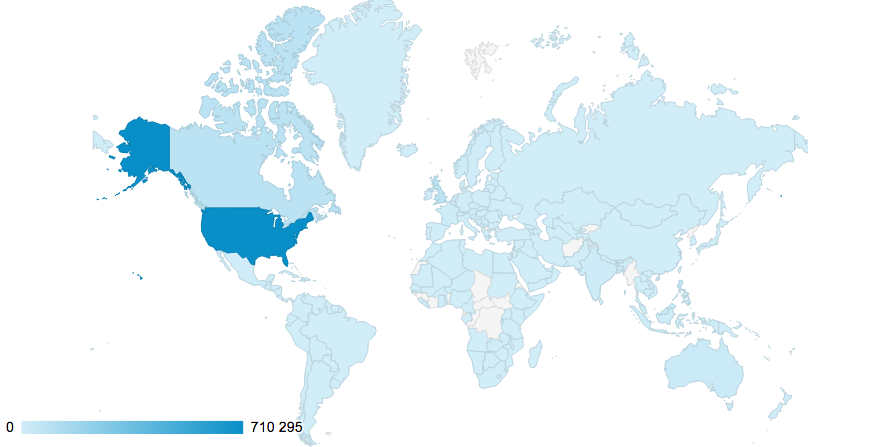
\includegraphics[width=400px]{images/visitesMondialesCarte.png}
		\caption{Visites depuis la création de Teen Quotes représentées sur une carte mondiale.}
	\end{figure}
	On a appliqué un dégradé de bleu pour symboliser le nombre de visites : le bleu foncé représentant le pays avec le plus de visiteurs.\\
	De cette carte on peut tirer l'analyse suivante :
	\vspace{10px}
	\begin{itemize}
		\item Quasiment tous les pays du monde sont coloriés en bleu : c'est-à-dire qu'il y a eu au moins une visite depuis 211 pays ou États\footnote{On obtient ce chiffre en regardant la liste des pays qui ont enregistré au moins une visite, et non en les comptant sur la carte !} dans le monde. Les pays grisés sont majoritairement situés en Afrique : l'absence de visites depuis ces pays peut s'expliquer par le faible taux d'accès à Internet pour les particuliers.
		\item Les visites depuis les États-Unis ont l'air très majoritaires, à tel point qu'il est difficile de voir une différence pour les autres visites tant les écarts sont grands entre le pays le plus visité et les autres.
	\end{itemize}
	\vspace{10px}
	Pour mieux visualiser le poids de chaque poids, représentons les visites sur un diagramme circulaire.
	\begin{figure}[H]
		\center
		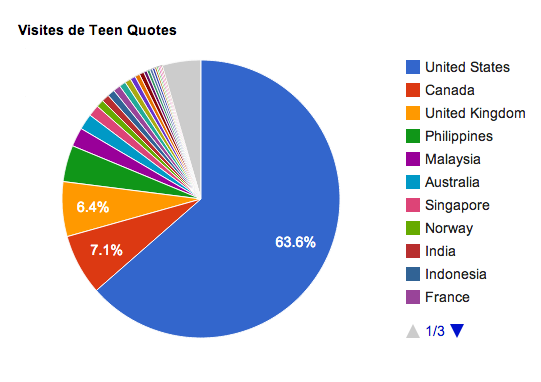
\includegraphics[width=250px]{images/visitesMondialesCamembert.png}
		\caption{Visites depuis la création de Teen Quotes représentées sur un diagramme circulaire.}
	\end{figure}
	La tendance observée précédemment est confirmée : les États-Unis sont de loin le pays qui génère le plus de visites. Plus impressionnant encore \textbf{le top 5 des pays (États-Unis, Canada, Royaume-Uni, Philippines et Malaisie) totalise 83,5 \% du total des visites}. Le reste des pays est très dispersé, contribuant chacun à environ 1 \% des visites.
	% ------------------------------------------ %
	% -- Plutôt smartphones ou ordinateurs ? --- %
	\section{Plutôt smartphones ou ordinateurs ?}
	On a vu précédemment que l'application pour iPhone / iTouch a été lancée en novembre 2012 alors que le site web et la version mobile ont été lancés en mai 2011. Pourquoi avoir attendu autant ? Tout simplement parce qu'il s'est avéré nécessaire en observant les données au fil du temps de posséder une telle application. Retour sur cette décision !\\

	Ici nous allons nous intéresser à l'évolution du nombre de visites par mois depuis un ordinateur, un mobile (smartphone ou tablette) et depuis l'application iPhone / iTouch quand celle-ci a été lancée.
	\begin{figure}[H]
		\center
		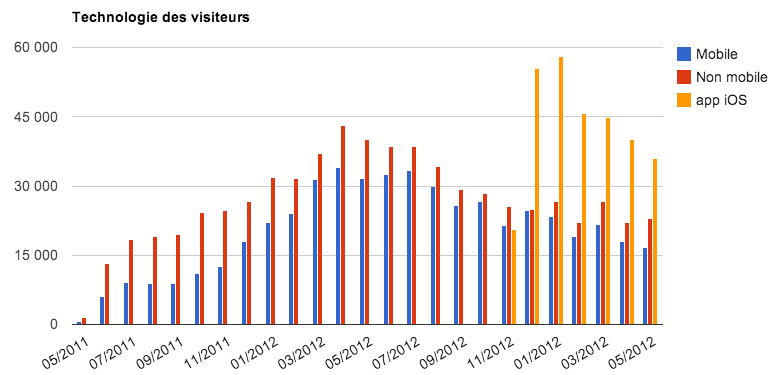
\includegraphics[width=500px]{images/visitesParAppareil.png}
		\caption{Visites mensuelles par type d'appareil.}
	\end{figure}
	Interprétons maintenant les résultats obtenus :
	\vspace{10px}
	\begin{itemize}
		\item Avant le lancement de l'application iOS on remarque qu'il y a quasiment autant de visiteurs depuis un appareil mobile que depuis un ordinateur. Cette statistique suit la montée du mobile dans les usages du web mais dans des proportions importantes : plus de 40 \% des visites se font depuis un smartphone ou une tablette. C'est cette statistique qui nous a poussé à réaliser une application iPhone / iTouch.
		\item Après le lancement de l'application iPhone / iTouch, pratiquement 50 \% des visites se font depuis l'application ! Le succès est grand. Le faible succès au mois de novembre 2012 s'explique par le lancement en fin de mois de l'application.
	\end{itemize}
	\vspace{10px}
	Maintenant, posons-nous la question : \textbf{pourquoi une application pour iOS et pas pour Android ou Windows Phone ?} Intéressons-nous aux systèmes d'exploitation mobiles qui ont navigué sur Teen Quotes.
	\begin{figure}[H]
		\center
		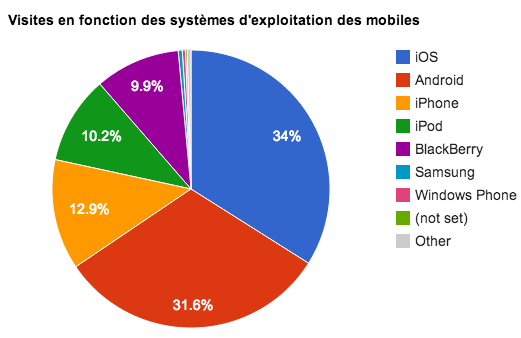
\includegraphics[width=300px]{images/OSMobiles.png}
		\caption{Visites en fonction des systèmes d'exploitation des mobiles.}
	\end{figure}
	En regardant ce diagramme, on pourrait penser que iOS est juste devant Android, sans une grande longueur d'avance. La subtilité réside dans le fait que le système d'exploitation des iPhone et iTouch est en réalité iOS : ces appareils annonçaient un nom différent il n'y a pas encore si longtemps. Il faut donc ajouter les pourcentages attribués aux systèmes d'exploitation iPhone et iTouch à iOS.\\

	Au final, on arrive à 57,1 \% des appareils mobiles sous iOS contre 31,6 \% des appareils mobiles sous Android. L'explication est donc là : \textbf{pour proposer une application qui répondait le plus aux attentes de nos visiteurs il fallait créer une application pour iOS}.
	\newpage
	% ---------------------------------------------- %
	% -- On ne passe pas assez de temps ensemble --- %
	\section{On ne passe pas assez de temps ensemble}
	Plus un visiteur reste longtemps, plus je suis content. J'aime bien quand les visiteurs prennent le temps de lire plusieurs citations voire plusieurs pages de citations ! Le top de mon bonheur étant bien sûr la création d'un compte voire même le remplissage d'un profil. Le comble du bonheur... Mais je m'éloigne du sujet il me semble : la durée moyenne de visite d'un visiteur de Teen Quotes.\\

	Observons donc l'évolution de la durée de visite moyenne d'un visiteur par mois depuis la création de Teen Quotes.
	\begin{figure}[H]
		\center
		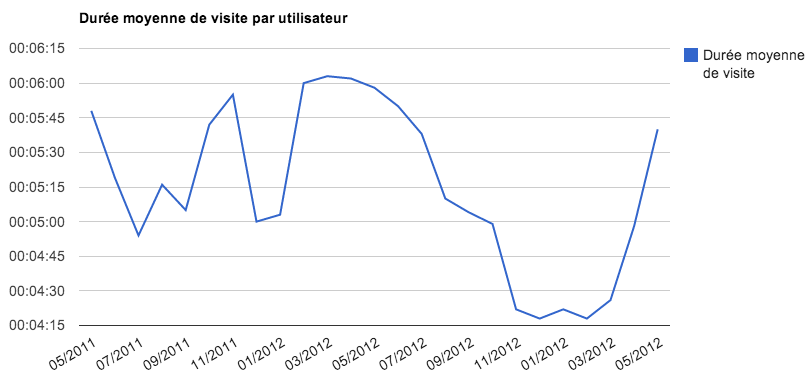
\includegraphics[width=500px]{images/dureeVisite.png}
		\caption{Durée de visite moyenne d'un visiteur.}
	\end{figure}
	On remarque immédiatement que la durée moyenne de visite la plus basse est de plus de 4 minutes et 15 secondes. C'est une excellente moyenne pour un site web ! Bonne nouvelle : Teen Quotes arrive à retenir les visiteurs pendant plusieurs minutes. N'oublions pas que plus de 40 \% des visites sont réalisées depuis un appareil mobile où la durée d'attention est généralement réduite.\\

	On remarque que les données sont assez éparpillées : il y a un écart de quasiment 2 minutes entre la valeur minimale et la valeur maximale ! Et 2 minutes de durée de visite en moyenne de différence sur une période d'un mois, c'est beaucoup. Je n'ai pas encore trouvé d'explication à ces écarts, je tâcherai de surveiller particulièrement ceci à l'avenir.

	% ------------------------------------- %
	% -- C'est un garçon ou une fille ? --- %
	\section{C'est un garçon ou une fille ?}
	J'ai bien peur d'avoir accouché de plusieurs million de filles. Enfin pas vraiment moi, mais plutôt Teen Quotes ! La connaissance de l'audience passe aussi par le genre des visiteurs : on ne proposera pas les mêmes citations à un public majoritairement féminin que masculin. Il est donc primordial de savoir quelle est la proportition de femmes et d'hommes dans notre audience.\\

	Les données proviennent des informations recueillies sur tous les utilisateurs de l'application iPhone / iTouch et des utilisateurs ne s'étant pas inscrits depuis l'application ayant renseigné leur sexe dans le profil de leur compte Teen Quotes. En effet, Flurry permet de connaître le sexe de l'utilisateur grâce aux informations de son compte Apple alors qu'il n'y a pas de moyen technique permettant d'identifier le sexe d'un visiteur naviguant sur le web !
	\begin{figure}[H]
		\center
		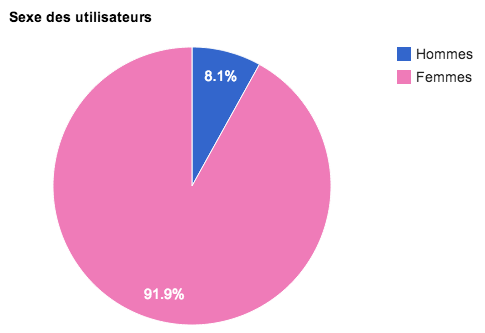
\includegraphics[width=300px]{images/sexeUtilisateurs.png}
		\caption{Proportion d'hommes et de femmes visitant Teen Quotes.}
	\end{figure}
	Wahou, c'est un non-match : il y a un paquet de filles. En y réfléchissant ceci peut se comprendre : les filles ont général plus besoin de se confier et de s'identifier que les garçons lors de la période de l'adolescence. Ça tombe bien, c'est exactement ce pourquoi a été créé Teen Quotes ! En plein dans le mille.

	% ///////////////////////////////////// %
	% /// Des citations, par milliers ///// %
	\chapter{Des citations, par milliers}
	Avant de s'attarder sur le coeur de Teen Quotes (les citations), il convient de rappeller les quelques subtilitées associées à celles-ci. Par commodité, on appelle les citations de Teen Quotes les \textbf{"quotes"}.
	\vspace{10px}
	\begin{itemize}
		\item Chaque utilisateur possédant un compte sur Teen Quotes peut soumettre 5 quotes par jour.
		\item Une fois une citation soumise, elle doit être acceptée avant d'être publiée. Une citation peut être acceptée telle qu'elle a été soumise ou légèrement modifiée.
		\item Tous les soirs à 0h (heure française), 5 nouvelles citations sont publiées.
		\item Il existe un système de "file d'attente" qui regroupe les citations en attente de publication : les citations ayant été approuvées les premières étant publiées en priorité.
	\end{itemize}

	% ----------------------------------------- %
	% -- Les statuts des quotes (Statu quo) --- %
	\section{Les statuts des quotes (\textit{Statu quo})}
	Intéressons-nous d'abord aux proportions des différents statuts de quotes.
	\begin{figure}[H]
		\center
		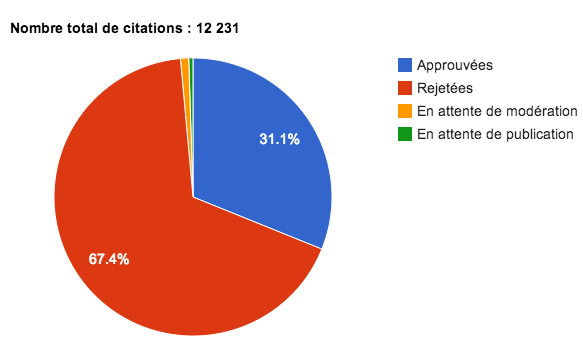
\includegraphics[width=330px]{images/statutsQuotes.png}
		\caption{Parts des différents statuts des quotes sur Teen Quotes.}
	\end{figure}
	On remarque qu'une majeure partie des citations ont été refusées. Ceci s'explique par le fait que Teen Quotes est aujourd'hui mature : beaucoup de citations sont soumises et l'objectif est de garder du contenu de haute qualité tout en évitant de publier des citations ayant déjà été publiées. À l'heure actuelle, la modération est donc plus stricte. Aujourd'hui, plus de 3 800 quotes ont été publiées sur Teen Quotes.

	60 quotes sont en attente de publication, ce qui signifie que le contenu est déjà prêt pour les 12 prochains jours. J'essaie de garder toujours une marge d'avance (environ 15 jours) pour le contenu qui sera publié, en cas d'imprévu personnel qui m'empêcherait de modérer des citations pendant une certaine période.

	Enfin, 117 quotes sont en attente de modération. Ce nombre de quotes en attente de modération est généralement atteint en 2 ou 3 jours sans effectuer de modération.\\

	Intéressons-nous maintenant aux différents statuts des citations, mais en fonction du temps. On fait seulement la distinction entre les citations approuvées et les citations refusées de la création de Teen Quotes jusqu'à une date donnée.
	\begin{figure}[H]
		\center
		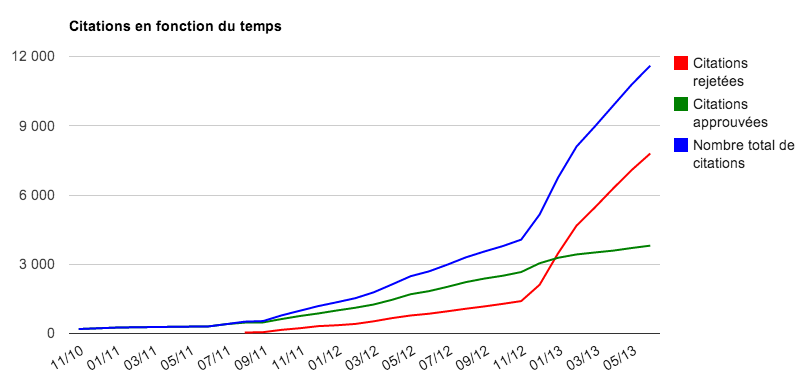
\includegraphics[width=450px]{images/statutsQuotesTemps.png}
		\caption{Nombre de citations acceptées et refusées en fonction du temps.}
	\end{figure}

	\begin{figure}[H]
		\center
		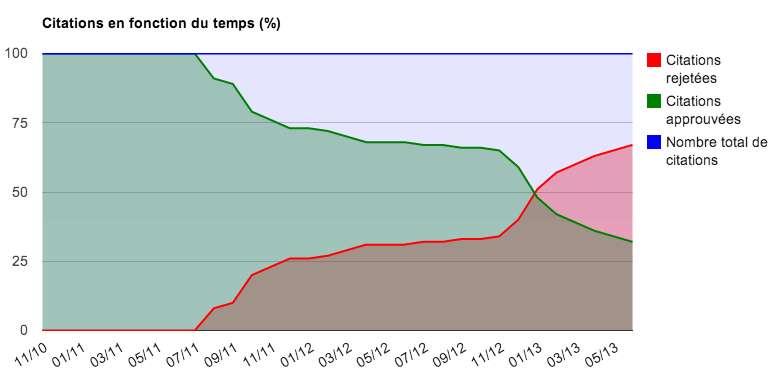
\includegraphics[width=450px]{images/statutsQuotesTempsPourcentage.png}
		\caption{Pourcentage de citations acceptées et refusées en fonction du temps.}
	\end{figure}
	
	La courbe (ou l'aire) bleue est la somme des courbes (ou des aires) bleues. 

	On remarque que la courbe verte est quasiment confondue avec la courbe bleue au lancement de Teen Quotes. Ceci s'explique par le fait qu'il était difficile de lancer Teen Quotes sans un contenu initial et une base d'utilisateurs quasi vide. Ainsi, il était habituel que je soumette et "m'auto-approuve" des quotes afin de proposer du contenu aux premiers visiteurs.\\

	Le nombre de quotes approuvées suit une croissance quasi linéaire depuis la création du site. En effet, le nombre de quotes postées par jour est quasiment constant à 5.\\

	En revanche, on remarque qu'à partir du mois de novembre 2012, le nombre de quotes refusées augmente énormément. Ceci s'explique par une hausse du nombre de soumissions de quotes (engendrée par une hausse du nombre de créations de comptes, mais nous le verrons plus loin !). Ce fort afflux de quotes a engendré beaucoup de refus car il n'était pas possible de publier toutes les quotes soumises. En conséquence, la modération des quotes soumises est très stricte depuis cette période car le nombre de quotes proposé est beaucoup plus important qu'auparavant.
% Fin du document
\end{document}